% Options for packages loaded elsewhere
\PassOptionsToPackage{unicode}{hyperref}
\PassOptionsToPackage{hyphens}{url}
\PassOptionsToPackage{dvipsnames,svgnames,x11names}{xcolor}
%
\documentclass[
]{article}

\usepackage{amsmath,amssymb}
\usepackage{iftex}
\ifPDFTeX
  \usepackage[T1]{fontenc}
  \usepackage[utf8]{inputenc}
  \usepackage{textcomp} % provide euro and other symbols
\else % if luatex or xetex
  \usepackage{unicode-math}
  \defaultfontfeatures{Scale=MatchLowercase}
  \defaultfontfeatures[\rmfamily]{Ligatures=TeX,Scale=1}
\fi
\usepackage{lmodern}
\ifPDFTeX\else  
    % xetex/luatex font selection
  \setmainfont[]{Latin Modern Roman}
  \setmathfont[]{Latin Modern Math}
\fi
% Use upquote if available, for straight quotes in verbatim environments
\IfFileExists{upquote.sty}{\usepackage{upquote}}{}
\IfFileExists{microtype.sty}{% use microtype if available
  \usepackage[]{microtype}
  \UseMicrotypeSet[protrusion]{basicmath} % disable protrusion for tt fonts
}{}
\makeatletter
\@ifundefined{KOMAClassName}{% if non-KOMA class
  \IfFileExists{parskip.sty}{%
    \usepackage{parskip}
  }{% else
    \setlength{\parindent}{0pt}
    \setlength{\parskip}{6pt plus 2pt minus 1pt}}
}{% if KOMA class
  \KOMAoptions{parskip=half}}
\makeatother
\usepackage{xcolor}
\setlength{\emergencystretch}{3em} % prevent overfull lines
\setcounter{secnumdepth}{5}
% Make \paragraph and \subparagraph free-standing
\ifx\paragraph\undefined\else
  \let\oldparagraph\paragraph
  \renewcommand{\paragraph}[1]{\oldparagraph{#1}\mbox{}}
\fi
\ifx\subparagraph\undefined\else
  \let\oldsubparagraph\subparagraph
  \renewcommand{\subparagraph}[1]{\oldsubparagraph{#1}\mbox{}}
\fi


\providecommand{\tightlist}{%
  \setlength{\itemsep}{0pt}\setlength{\parskip}{0pt}}\usepackage{longtable,booktabs,array}
\usepackage{calc} % for calculating minipage widths
% Correct order of tables after \paragraph or \subparagraph
\usepackage{etoolbox}
\makeatletter
\patchcmd\longtable{\par}{\if@noskipsec\mbox{}\fi\par}{}{}
\makeatother
% Allow footnotes in longtable head/foot
\IfFileExists{footnotehyper.sty}{\usepackage{footnotehyper}}{\usepackage{footnote}}
\makesavenoteenv{longtable}
\usepackage{graphicx}
\makeatletter
\def\maxwidth{\ifdim\Gin@nat@width>\linewidth\linewidth\else\Gin@nat@width\fi}
\def\maxheight{\ifdim\Gin@nat@height>\textheight\textheight\else\Gin@nat@height\fi}
\makeatother
% Scale images if necessary, so that they will not overflow the page
% margins by default, and it is still possible to overwrite the defaults
% using explicit options in \includegraphics[width, height, ...]{}
\setkeys{Gin}{width=\maxwidth,height=\maxheight,keepaspectratio}
% Set default figure placement to htbp
\makeatletter
\def\fps@figure{htbp}
\makeatother
\newlength{\cslhangindent}
\setlength{\cslhangindent}{1.5em}
\newlength{\csllabelwidth}
\setlength{\csllabelwidth}{3em}
\newlength{\cslentryspacingunit} % times entry-spacing
\setlength{\cslentryspacingunit}{\parskip}
\newenvironment{CSLReferences}[2] % #1 hanging-ident, #2 entry spacing
 {% don't indent paragraphs
  \setlength{\parindent}{0pt}
  % turn on hanging indent if param 1 is 1
  \ifodd #1
  \let\oldpar\par
  \def\par{\hangindent=\cslhangindent\oldpar}
  \fi
  % set entry spacing
  \setlength{\parskip}{#2\cslentryspacingunit}
 }%
 {}
\usepackage{calc}
\newcommand{\CSLBlock}[1]{#1\hfill\break}
\newcommand{\CSLLeftMargin}[1]{\parbox[t]{\csllabelwidth}{#1}}
\newcommand{\CSLRightInline}[1]{\parbox[t]{\linewidth - \csllabelwidth}{#1}\break}
\newcommand{\CSLIndent}[1]{\hspace{\cslhangindent}#1}

\usepackage{booktabs}
\usepackage{longtable}
\usepackage{array}
\usepackage{multirow}
\usepackage{wrapfig}
\usepackage{float}
\usepackage{colortbl}
\usepackage{pdflscape}
\usepackage{tabu}
\usepackage{threeparttable}
\usepackage{threeparttablex}
\usepackage[normalem]{ulem}
\usepackage{makecell}
\usepackage{xcolor}
\usepackage{tipa}
\usepackage{booktabs}
\usepackage{arxiv}
\usepackage{orcidlink}
\usepackage{amsmath}
\usepackage[T1]{fontenc}
\makeatletter
\makeatother
\makeatletter
\makeatother
\makeatletter
\@ifpackageloaded{caption}{}{\usepackage{caption}}
\AtBeginDocument{%
\ifdefined\contentsname
  \renewcommand*\contentsname{Table of contents}
\else
  \newcommand\contentsname{Table of contents}
\fi
\ifdefined\listfigurename
  \renewcommand*\listfigurename{List of Figures}
\else
  \newcommand\listfigurename{List of Figures}
\fi
\ifdefined\listtablename
  \renewcommand*\listtablename{List of Tables}
\else
  \newcommand\listtablename{List of Tables}
\fi
\ifdefined\figurename
  \renewcommand*\figurename{Figure}
\else
  \newcommand\figurename{Figure}
\fi
\ifdefined\tablename
  \renewcommand*\tablename{Table}
\else
  \newcommand\tablename{Table}
\fi
}
\@ifpackageloaded{float}{}{\usepackage{float}}
\floatstyle{ruled}
\@ifundefined{c@chapter}{\newfloat{codelisting}{h}{lop}}{\newfloat{codelisting}{h}{lop}[chapter]}
\floatname{codelisting}{Listing}
\newcommand*\listoflistings{\listof{codelisting}{List of Listings}}
\makeatother
\makeatletter
\@ifpackageloaded{caption}{}{\usepackage{caption}}
\@ifpackageloaded{subcaption}{}{\usepackage{subcaption}}
\makeatother
\makeatletter
\@ifpackageloaded{tcolorbox}{}{\usepackage[skins,breakable]{tcolorbox}}
\makeatother
\makeatletter
\@ifundefined{shadecolor}{\definecolor{shadecolor}{rgb}{.97, .97, .97}}
\makeatother
\makeatletter
\makeatother
\makeatletter
\makeatother
\ifLuaTeX
  \usepackage{selnolig}  % disable illegal ligatures
\fi
\IfFileExists{bookmark.sty}{\usepackage{bookmark}}{\usepackage{hyperref}}
\IfFileExists{xurl.sty}{\usepackage{xurl}}{} % add URL line breaks if available
\urlstyle{same} % disable monospaced font for URLs
\hypersetup{
  colorlinks=true,
  linkcolor={blue},
  filecolor={Maroon},
  citecolor={Blue},
  urlcolor={Blue},
  pdfcreator={LaTeX via pandoc}}

\usepackage{lineno}
\linenumbers
\newcommand{\runninghead}{A Preprint }
\renewcommand{\runninghead}{Cognate beginnings to bilingual lexical
acquistion (Appendix) }
\author{}
\date{}
\begin{document}
\ifdefined\Shaded\renewenvironment{Shaded}{\begin{tcolorbox}[interior hidden, borderline west={3pt}{0pt}{shadecolor}, enhanced, breakable, sharp corners, boxrule=0pt, frame hidden]}{\end{tcolorbox}}\fi

\hypertarget{appendix-a-frequency-and-language-exposure-as-separate-predictors}{%
\section*{Appendix A: frequency and language exposure as separate
predictors}\label{appendix-a-frequency-and-language-exposure-as-separate-predictors}}
\addcontentsline{toc}{section}{Appendix A: frequency and language
exposure as separate predictors}

As a robustness check, we fit a model similar to the one described in
the main manuscript, but including lexical frequency and language degree
of exposure as separate predictors, instead of the composite measure
\emph{Exposure}. Language degree of exposure (\emph{DoE}) was included
in interaction with \emph{Age} and \emph{Cognateness}, while lexical
frequency (\emph{Frequency}) was included as a main effect.
Table~\ref{tbl-coefs-doe} shows a comparison between the posterior
distribution of the regression coefficients of both models. Overall,
results are equivalent.

\begin{table}

\caption{\label{tbl-coefs-doe}\textbf{?(caption)}}\begin{minipage}[t]{\linewidth}
\subcaption{\label{tbl-coefs-doe-1}}

{\centering 

\begin{tabular}{lclrl}
\toprule
 & $\beta$ & 95\% HDI & $p(\text{ROPE})$ & \\
\midrule
\addlinespace[0.3em]
\multicolumn{5}{l}{\textbf{Model: Exposure}}\\
\hspace{1em}Age (+1 SD, 4.87, months) & 0.600 & {}[0.588, 0.611] & .000 & \\
\hspace{1em}Exposure (+1 SD, 1.81) & 0.558 & {}[0.55, 0.567] & .000 & \\
\hspace{1em}Cognateness (+1 SD, 0.26) & 0.515 & {}[0.504, 0.526] & .037 & \\
\hspace{1em}Length (+1 SD, 1.56 phonemes) & 0.485 & {}[0.478, 0.491] & .000 & \\
\hspace{1em}Age $\times$ Exposure & 0.518 & {}[0.51, 0.526] & .000 & \\
\hspace{1em}Age $\times$ Cognateness & 0.504 & {}[0.5, 0.506] & .985 & \\
\hspace{1em}Exposure $\times$ Cognateness & 0.486 & {}[0.483, 0.488] & .000 & \\
\hspace{1em}Age $\times$ Exposure $\times$ Cognateness & 0.495 & {}[0.493, 0.498] & .975 & \\
\addlinespace[0.3em]
\multicolumn{5}{l}{\textbf{Model: Frequency \& DoE}}\\
\hspace{1em}Age (+1 SD, 4.87, months) & 0.601 & {}[0.59, 0.612] & .000 & \\
\hspace{1em}DoE (+1 SD, 0.3) & 0.558 & {}[0.549, 0.566] & .000 & \\
\hspace{1em}Cognateness (+1 SD, 0.26) & 0.516 & {}[0.506, 0.528] & .016 & \\
\hspace{1em}Phonemes (+1 SD, 1.56 phonemes) & 0.486 & {}[0.479, 0.492] & .000 & \\
\hspace{1em}Frequency (+1 SD, 0.19) & 0.527 & {}[0.516, 0.54] & .000 & \\
\hspace{1em}Age $\times$ DoE & 0.518 & {}[0.51, 0.527] & .000 & \\
\hspace{1em}Age $\times$ Cognateness & 0.504 & {}[0.501, 0.507] & .954 & \\
\hspace{1em}DoE $\times$ Cognateness & 0.486 & {}[0.483, 0.488] & .000 & \\
\hspace{1em}Age $\times$ DoE $\times$ Cognateness & 0.495 & {}[0.493, 0.498] & .962 & \\
\bottomrule
\end{tabular}

}

\end{minipage}%
\newline
\begin{minipage}[t]{\linewidth}

{\centering 

Posterior distribution of regression coefficients of the model including
the \emph{Exposure} composite predictor, and of the model including
lexical frequency (\emph{Frequency}) and degree of exposure (\emph{DoE})
separately. Median: median of the posterior distribution in the
probability scale. 95\% HDI: 95\% highest density interval of the
distribution. p(ROPE): overlap between the 95\% HDI and the ROPE,
indicating the posterior probability that the true value of the
coefficient is equivalent to zero. In the right column, we show a
graphical representation of the median and 95\% HDI of each coefficient,
with a reference dotted line indicating the location of zero.

}

\end{minipage}%

\end{table}

\newpage{}

\hypertarget{appendix-b-frequency-and-language-exposure-as-separate-predictors}{%
\section*{Appendix B: frequency and language exposure as separate
predictors}\label{appendix-b-frequency-and-language-exposure-as-separate-predictors}}
\addcontentsline{toc}{section}{Appendix B: frequency and language
exposure as separate predictors}

We define syllable frequency as the rate of appearance of individual
syllables in the word-forms included in the Barcelona Vocabulary
Questionnaire (BVQ)
(\protect\hyperlink{ref-garcia-castro2023bvq}{Garcia-Castro et al.,
2023}). Each item corresponds to a Catalan or Spanish word, and has an
associated phonological transcription in X-SAMPA format
(\protect\hyperlink{ref-wells1995computercoding}{Wells, 1995}). These
transcriptions are syllabified. Some examples:

\hypertarget{tbl-syll-items}{}
\begin{table}
\caption{\label{tbl-syll-items}Sample of items included in the BVQ questionnaire and their syllabified
SAMPA transcriptions in Catalan and Spanish }\tabularnewline

\centering
\begin{tabular}{lllcllc}
\toprule
Translation & Item & X-SAMPA & Syllables & Item & X-SAMPA & Syllables\\
\midrule
ladybug & marieta & m@.4i"E.t@ & 4 & mariquita & ma.4i"ki.ta & 4\\
beans & mongetes & muJ"ZE.t@s & 3 & alubias & a"lu.bjas & 3\\
tongue & llengua & "LeN.gw@ & 2 & lengua & "len.gwa & 2\\
kitchen & cuina & "kuj.n@ & 2 & cocina & ko"Ti.na & 3\\
cheek & galta & "ga5.t@ & 2 & mejilla & me"xi.La & 3\\
\addlinespace
purse & bossa & "bo.s@ & 2 & bolso & "bol.so & 2\\
farm & granja & g4aJ.Z@ & 2 & granja & "g4an.xa & 2\\
sausage & salsitxa & s@5"si.t͡S@ & 3 & salchicha & sal"tSi.tSa & 3\\
cereal & cereals & s@.4e"a5s & 3 & cereales & Te.4e"a.les & 4\\
bottle & ampolla & @m"po.L@ & 3 & botella & bo"te.La & 3\\
\addlinespace
boat & vaixell & b@"SeL & 2 & barco & "ba4.ko & 2\\
family & família & fa"mi.lia & 3 & familia & fa"mi.lia & 3\\
balloon & globus & "g5O.Bus & 2 & globo & "glo.Bo & 2\\
bee & abella & @"BE.L@ & 3 & abeja & a"Be.xa & 3\\
earring & arracada / arracades & @.r@"ka.D@ & 4 & pendientes & pen"Djen.tes & 3\\
\bottomrule
\end{tabular}
\end{table}

Most Catalan and Spanish words had two syllables, with Spanish words
having three and four syllables more often than Catalan words. Less than
1\% of the words included in the analyses presented in the main body of
the manuscripts had five syllables. No words had more than five
syllables (see Figure~\ref{fig-syll-number}). We extracted lexical
frequencies from the English corpora in the CHILDES database
(\protect\hyperlink{ref-macwhinney2000childes}{MacWhinney, 2000};
\protect\hyperlink{ref-sanchez2019childesdb}{Sanchez et al., 2019}).
Using the Catalan and Spanish corpora was not possible due to the low
number of children and tokens included in the corpora.

\begin{figure}

{\centering 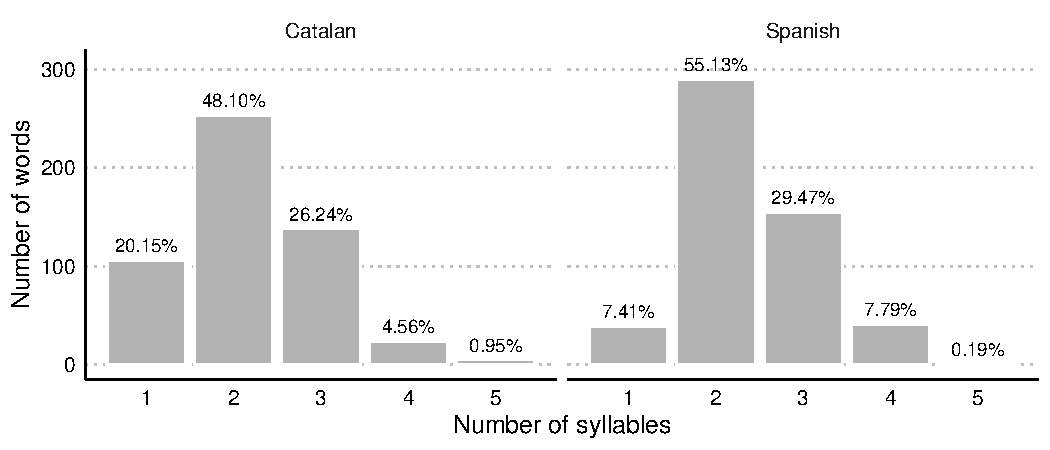
\includegraphics{appendix_files/figure-pdf/fig-syll-number-1.pdf}

}

\caption{\label{fig-syll-number}Distribution of the number of syllables
in Catalan and Spanish}

\end{figure}

We now present how syllable frequencies were calculated. Every exposure
to a word-form also counts as a exposure to each of the syllables that
make up such word. Every time a child hears the word \emph{casa}
{[}house{]}, they are exposed to the syllables \emph{ca} and \emph{sa}.
Syllables that appear embedded in words with higher lexical frequency
will also be more frequent. To compute the relative frequency of each
syllable in Catalan and Spanish (i.e., how many times the syllables
appears in every million words in Catalan or Spanish speech), we summed
the relative lexical frequency in CHILDES of every word that contains
such syllable in the corresponding language. Figure~\ref{fig-syll-freq}
shows the distribution of frequencies across syllables in Catalan and
Spanish. In the log10 scale, syllable frequencies in Catalan and Spanish
followed a slightly asymmetric distribution, with most syllables scoring
around 1,000 counts per million, and a longer tail to the right of the
distribution.

\begin{figure}

{\centering 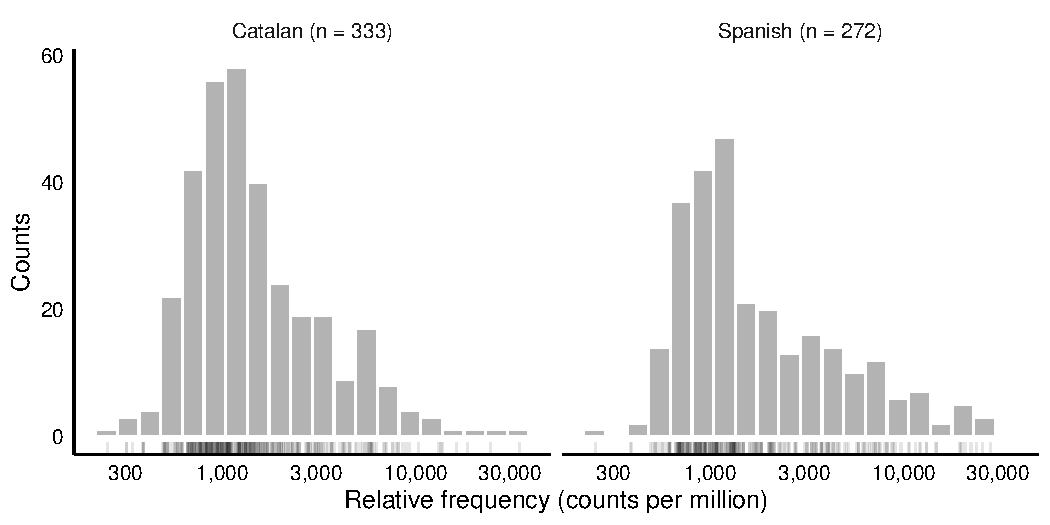
\includegraphics{appendix_files/figure-pdf/fig-syll-freq-1.pdf}

}

\caption{\label{fig-syll-freq}Distribution of apositional syllable
frequencies in Spanish and Catalan}

\end{figure}

To estimate the association between word-level syllabic frequency and
cognateness, while controlling for the number of syllables in the word,
as words are expected to necessarily increase the syllabic frequency of
the word), we fit a multilevel, Bayesian linear regression model with
syllabic frequency (the sum of the syllabic frequency of the syllables
in a word) as response variable, and the main effect of the number of
syllables (\(Syllables\)) and \(Cognateness\) (Levenshtein similarity
between a word and its translation equivalent,
\protect\hyperlink{ref-levenshtein1966binary}{Levenshtein, 1966}) as
predictors. We added translation equivalent-level random effects for the
intercept and the main effect of \(Syllables\) (some translation pairs
had a different number of syllables in each language). We used a
Gaussian distribution to model syllabic frequency scores after
standardising this variable and the predictors. We used a weakly
informative prior for all parameters involved in the model (see
Equation~\ref{eq-model-syllables} for a formal equation of this model
and its prior). We conducted statistical inference by evaluating the
proportion of the 95\% highest density interval (HDI) of the posterior
posterior distribution of each coefficient that fell into the region of
practical equivalence (ROPE, see the main manuscript for a more detailed
explanation, \protect\hyperlink{ref-kruschke2018bayesian}{Kruschke \&
Liddell, 2018}).

\begin{equation}\protect\hypertarget{eq-model-syllables}{}{
\begin{aligned}
\text{Syllable frequency} &\sim \mathcal{N}(\mu, \sigma)\\
\mu &= (\beta_0 + u_{0_{i}}) + (\beta_1 + u_{1_{i}}) \text{Syllables} + \beta_2 \text{Cognateness} \\
\beta_{0-3} &\sim \mathcal{N}(0, 10) \\
u_{{0-1}_{i}} &\sim \mathcal{N}(0, \sigma_{u_i}) \\
\sigma_y & \sim \text{Exponential}(2)\\
\Big(\begin{smallmatrix}
u_{0_{i}} \\ 
u_{1_{i}} \\ 
\end{smallmatrix}\Big) &\sim \mathcal{N} 
\Big(\Big(\begin{smallmatrix}0 \\
0\end{smallmatrix}\Big), \Sigma_{u}\Big) \\
\Sigma_{u} &= \Big(\begin{smallmatrix} \\
\sigma_{u_{0}} & \rho_{u_{0}} \sigma_{u_{0}} \sigma_{u_{1}} \\ 
\rho_{u_{1}} \sigma_{u_{1}} \sigma_{u_{0}} & \sigma_{u_{1}} \end{smallmatrix}\Big) \\
\sigma_{u_{0-1}} &\sim \mathcal{N_{+}}(1, 0.1) \\
\rho_{u} &\sim LKJcorr(2) \\
\end{aligned}
}\label{eq-model-syllables}\end{equation}

We fit this model running 4 sampling chains with 1,000 iterations each.
Table~\ref{tbl-syll-coefs} shows a summary of the posterior distribution
of the fixed effects in the model. As expected, words with more
syllables scored higher in syllabic frequency: all posterior draws for
the regression coefficient of the main effect of this predictor fell
outside the ROPE defined between -0.5 and +0.5 (\(\beta\) = 5.64, 95\%
HDI = {[}5.58, 5.71{]}). Keeping the number of syllables constant, the
effect of cognateness was negligible: all of the posterior distributions
of this predictor fell within the ROPE, providing evidence that the true
value of the increment in syllabic frequency for every increase in
cognateness is equivalent to zero (\(\beta\) = 0.01, 95\% HDI =
{[}-0.06, 0.07{]}).

\hypertarget{tbl-syll-coefs}{}
\begin{table}
\caption{\label{tbl-syll-coefs}Posterior distribution of regression coefficients. }\tabularnewline

\centering
\begin{tabular}{lclr>{}c}
\toprule
 & $\beta$ & 95\% HDI & $p(\text{ROPE})$ & \\
\midrule
Intercept & 16.089 & {}[16.023, 16.163] & .000 & \cellcolor[HTML]{f2f2f2}{}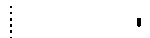
\includegraphics[width=1in, height=0.25in]{C:/Users/u155880/Documents/cognate-beginnings/appendix_files/figure-latex/pointrange_1e8078876ee9.pdf}\\
Syllables (+1 SD, 0.802) & 5.642 & {}[5.577, 5.711] & .000 & \cellcolor[HTML]{f2f2f2}{}
\includegraphics[width=1in, height=0.25in]{C:/Users/u155880/Documents/cognate-beginnings/appendix_files/figure-latex/pointrange_1e807c1b3ef.pdf}\\
Cognateness (+1 SD, 0.24) & 0.007 & {}[-0.059, 0.075] & 1.000 & \cellcolor[HTML]{f2f2f2}{}
\includegraphics[width=1in, height=0.25in]{C:/Users/u155880/Documents/cognate-beginnings/appendix_files/figure-latex/pointrange_1e8043796412.pdf}\\
\bottomrule
\end{tabular}
\end{table}

Figure~\ref{fig-syll-marginal} shows the median posterior-predicted
syllabic frequencies for words with one to four syllables, for the whole
range of cognateness values. Overall, cognate words' syllabic frequency
is equivalent to that of non-cognates. This suggests that the cognate
facilitation effect in word acquisition reported in the present study is
not the result from an association between cognateness and higher
syllabic frequencies.

\begin{figure}

{\centering 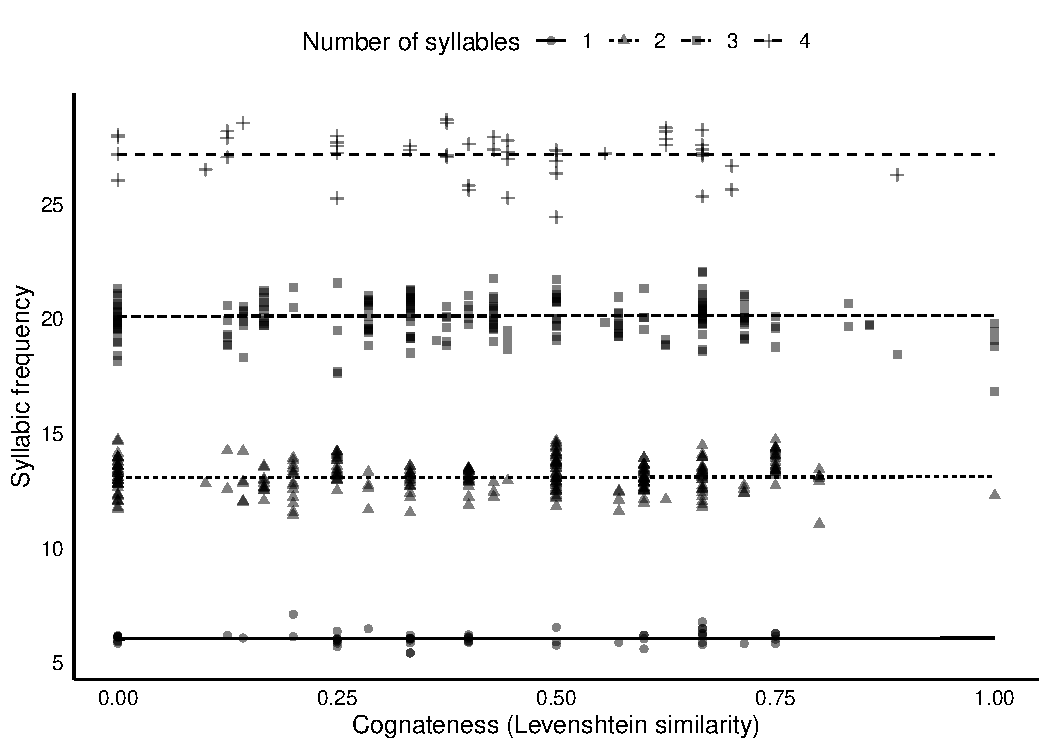
\includegraphics[width=0.8\textwidth,height=\textheight]{appendix_files/figure-pdf/fig-syll-marginal-1.pdf}

}

\caption{\label{fig-syll-marginal}Posterior-predictions of the syllabic
frequency model. Thicker lines indicate the median of the posterior
predictions, and thinner lines indicate individual posterior
predictions.}

\end{figure}

\newpage{}

\hypertarget{references}{%
\section*{References}\label{references}}
\addcontentsline{toc}{section}{References}

\hypertarget{refs}{}
\begin{CSLReferences}{1}{0}
\leavevmode\vadjust pre{\hypertarget{ref-garcia-castro2023bvq}{}}%
Garcia-Castro, G., Ávila-Varela, D. S., \& Sebastian-Galles, N. (2023).
\emph{Bvq: Barcelona vocabulary questionnaire database and helper
functions}. \url{https://gongcastro.github.io/bvq}

\leavevmode\vadjust pre{\hypertarget{ref-kruschke2018bayesian}{}}%
Kruschke, J. K., \& Liddell, T. M. (2018). The bayesian new statistics:
Hypothesis testing, estimation, meta-analysis, and planning from a
bayesian perspective. \emph{Psychonomic Bulletin \&Review}, \emph{25},
178--206. \url{https://doi.org/10.3758/s13423-016-1221-4}

\leavevmode\vadjust pre{\hypertarget{ref-levenshtein1966binary}{}}%
Levenshtein, V. I. (1966). Binary codes capable of correcting deletions,
insertions, and reversals. \emph{Soviet Physics-Doklady}, \emph{10},
707--710.

\leavevmode\vadjust pre{\hypertarget{ref-macwhinney2000childes}{}}%
MacWhinney, B. (2000). \emph{The {CHILDES} project: The database} (Vol.
2). Psychology Press.

\leavevmode\vadjust pre{\hypertarget{ref-sanchez2019childesdb}{}}%
Sanchez, A., Meylan, S. C., Braginsky, M., MacDonald, K. E., Yurovsky,
D., \& Frank, M. C. (2019). Childes-db: A flexible and reproducible
interface to the child language data exchange system. \emph{Behavior
Research Methods}, \emph{51}(4), 1928--1941.

\leavevmode\vadjust pre{\hypertarget{ref-wells1995computercoding}{}}%
Wells, J. C. (1995). \emph{Computer-coding the {IPA}: A proposed
extension of {SAMPA}}. \emph{4}(28), 1995.

\end{CSLReferences}



\end{document}
